\section{Controller Optimization}

Given the physical simulation, we can design controllers to enable the robot to achieve various locomotion tasks in the simulated environment. The three tasks that we use to test our system are rising from a leaning, sitting or kneeling position to an erect stance (Figure \ref{fig:task}). For each task, the joint configuration of the initial pose and the final pose are provided by the user. The goal of controller optimization is to find a sequence of control signals $\bar{q}(t)$ so that the robot can move from the initial to the final pose without losing balance. We purposefully choose to use only feedforward controllers\footnote{There is still an internal feedback loop in the actuators to track the desired joint angle (See Chapter~\ref{sec:motorDynamics}). However, this feedback loop is not fully programmable.} in this work, which means that the control signal $\bar{\mathbf{q}}(t)$ is a only function of time $t$ and does not depend on the states of the robot. With the feedforward control alone, the controller transfer can only succeed if the simulation is close enough to the real-world environment. This will put the simulation calibration subsystem into more thorough tests.

\begin{figure*}[!t]
  \centering
  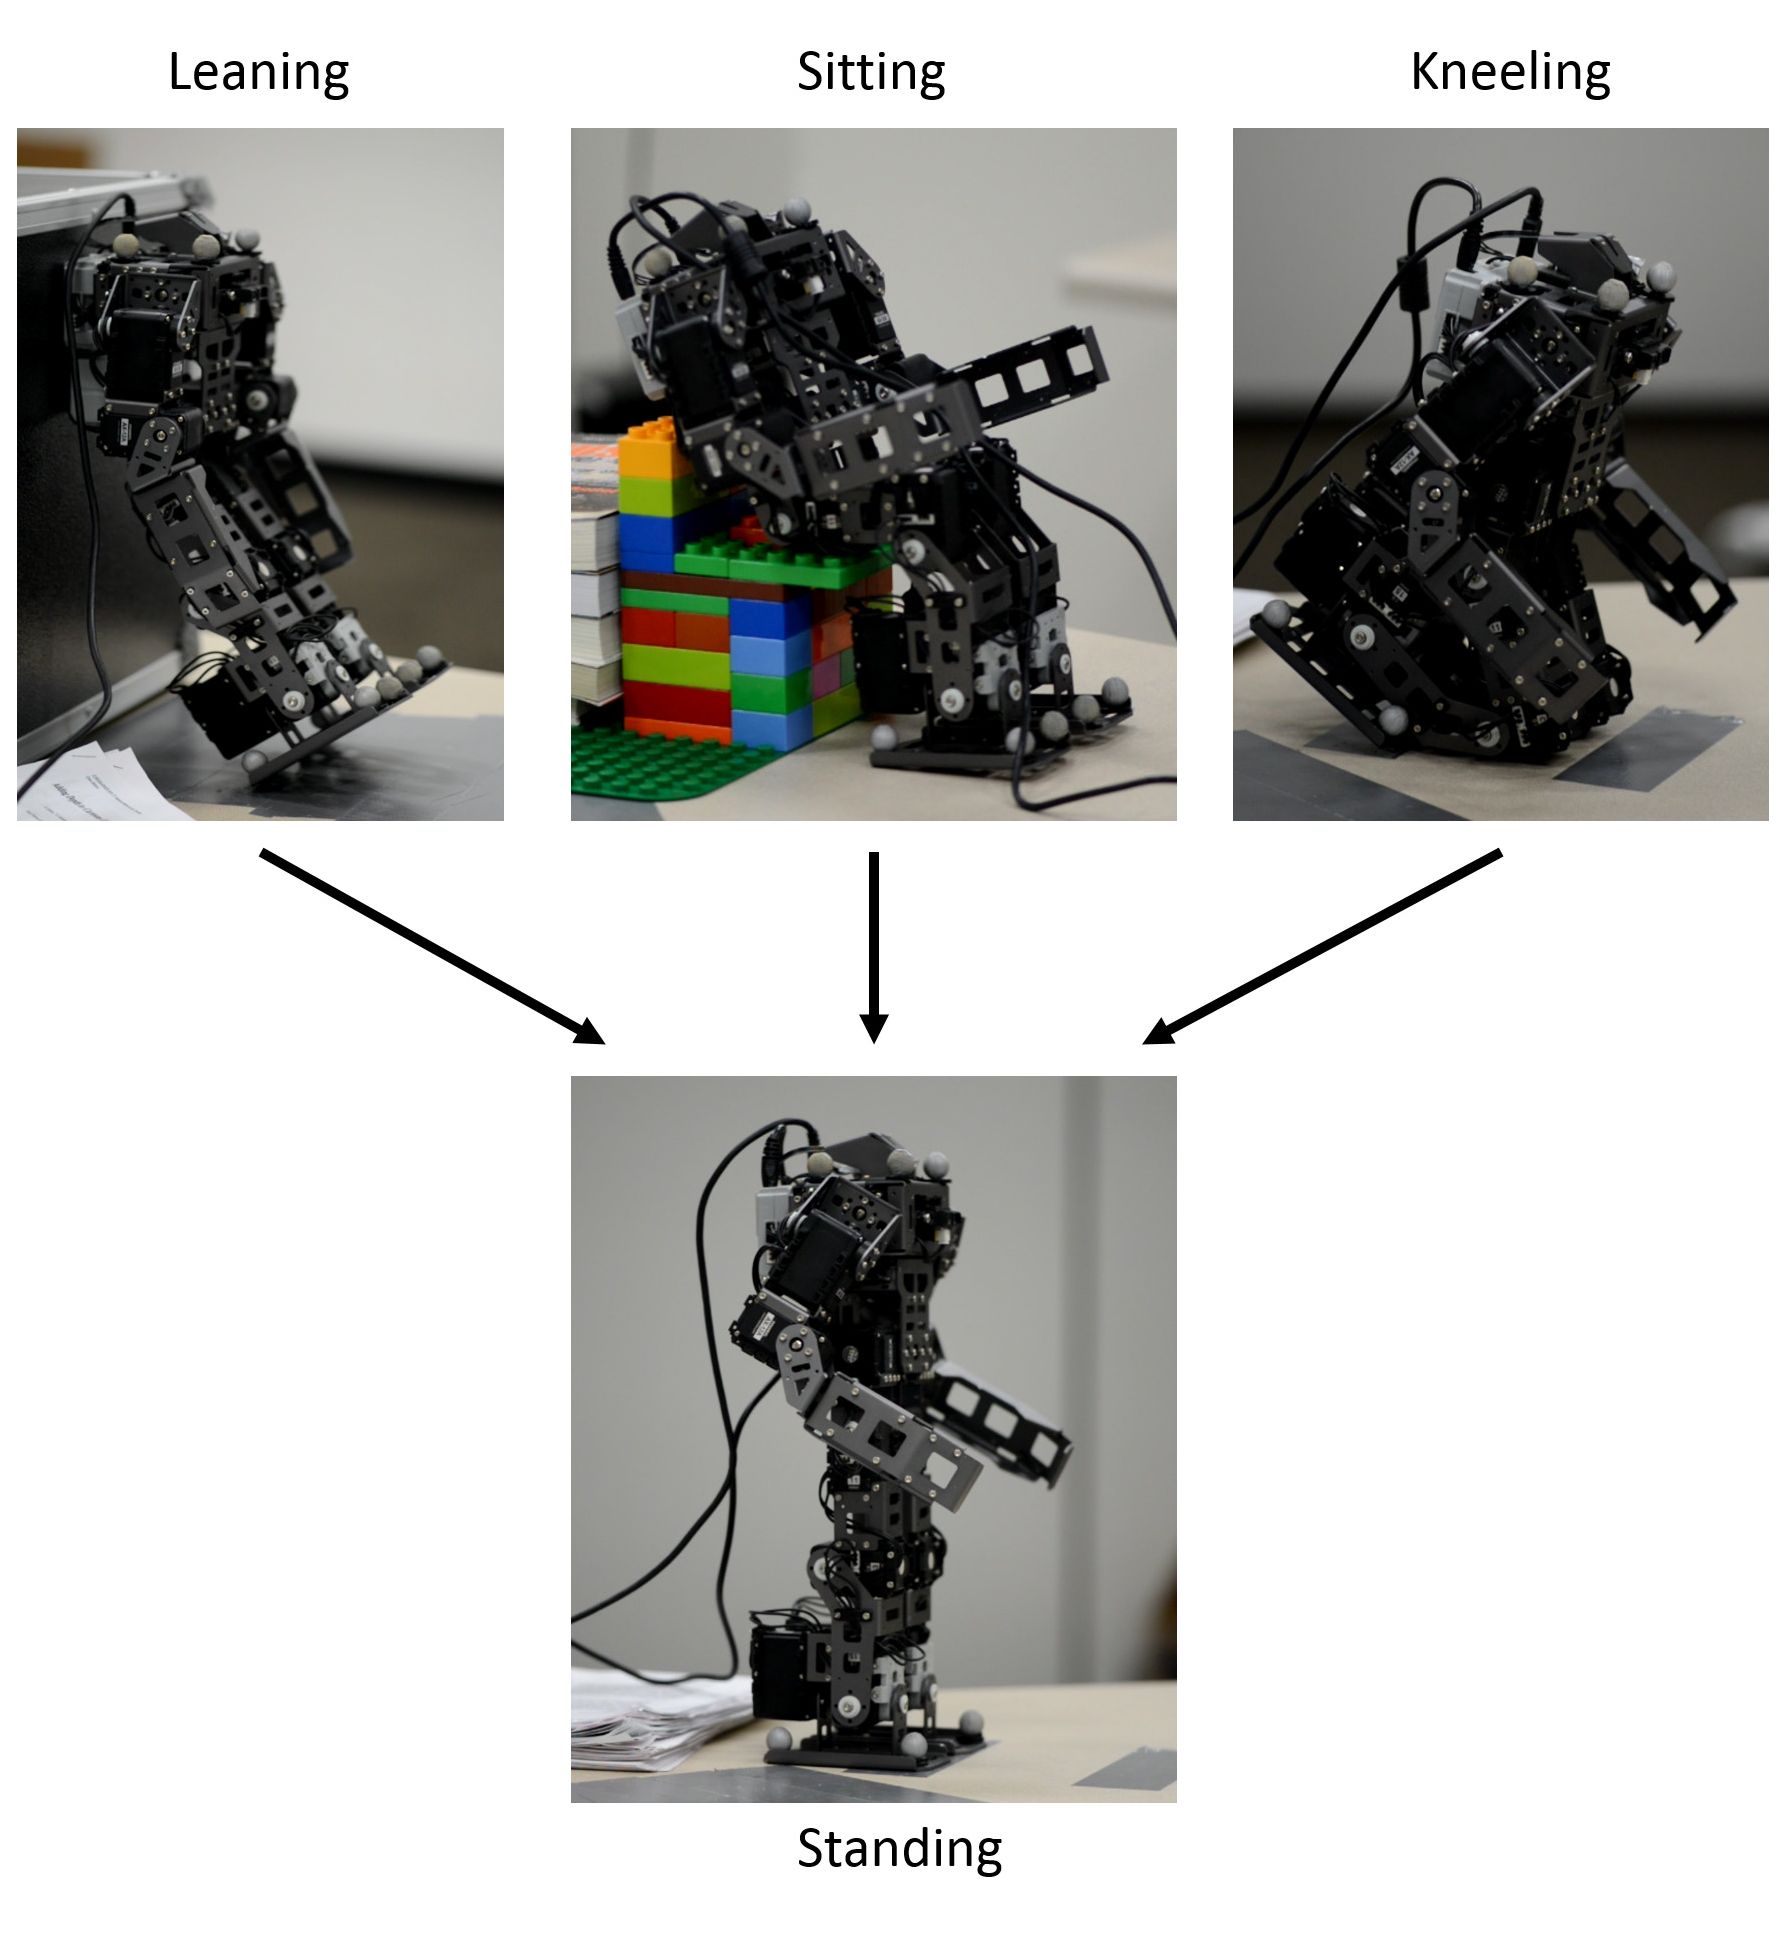
\includegraphics[width=0.7\textwidth]{figures/initialFinal}
  \caption{The initial and the final joint configurations of the locomotion tasks. Top row: the initial poses of leaning, sitting and kneeling. Bottom row: the final standing pose for all three tasks.}
  \label{fig:task}
\end{figure*}


We first formulate a trajectory optimization problem for each task.
\begin{align}
 \label{eqn:obj}&\max_{\bar{\mathbf{q}}(t),T} V_{ctrl}(\mathbf{x}(t))\\
\nonumber  \mathrm{subject\;} &\mathrm{to} \\
\label{eqn:dyn1} & \mathbf{M}(\mathbf{x})\mathbf{\ddot{x}}+\mathbf{C}(\mathbf{x},\mathbf{\dot{x}}) =\tau + \mathbf{J}^T\mathbf{f}\\
\label{eqn:dyn2} &\tau =
  \left\{
    \begin{array}{ll}
      \tau_{min} & \text{if }\tau < \tau_{min},\\
      \tau_{max} & \text{if }\tau > \tau_{max},\\
      -k_p(\mathbf{q}-\bar{\mathbf{q}}) - k_d\dot{\mathbf{q}} - k_c\sgn(\dot{\mathbf{q}}) & \text{otherwise.}\\
    \end{array}
  \right.\\
\label{eqn:boundary1}&\bar{\mathbf{x}}(0) = \mathbf{x}_0\\
\label{eqn:boundary2}&\bar{\mathbf{q}}(t) = \mathbf{q}_T, \text{if } t \geq T
\end{align}

This optimization searches for the duration $T$ of the rising motion and the trajectory of the desired joint configuration $\bar{\mathbf{q}}(t)$ to maximize a task-related fitness function $V_{ctrl}$, and subject to physical constraints (eq.(\ref{eqn:dyn1}) and (\ref{eqn:dyn2})) and boundary conditions (eq.(\ref{eqn:boundary1}) and (\ref{eqn:boundary2})). $\mathbf{x}_0$ is the initial condition, and $\mathbf{q}_T$ is the final pose (Figure \ref{fig:task}), both of which are provided by the user. Note that although we can specify the global translation $\mathbf{p}_0$, rotation $\mathbf{r}_0$ and joint angles $\mathbf{q}_0$ in the initial condition, we can only specify the desired joint angles for the final pose because the global translation and rotation are determined by the physical simulation.

Assuming no interbody collision happens when the robot executes $\bar{\mathbf{q}}(t)$, in our tasks, the robot can alway reach the final pose $\mathbf{q}_T$ within a small error due to the weight of the bodies that each actuator supports. The criterion of success for all the tasks is whether the robot remains upright at the end of its motion. We use the following fitness function to reward controllers that keep balance throughout the entire motion.

\begin{equation}
  V_{ctrl}(\mathbf{x}(t))=\int_0^{T+1} \frac{1}{\alpha(t)+\epsilon}\mathrm{d}t
  \label{eqn:controllerObj}
\end{equation}
where $\alpha(t)$ is the angle between the up direction in the local frame of the robot's torso and the up direction in the global frame $(0,0,1)$. It measures how far the robot is to losing its balance. $\epsilon$ is a small positive number to prevent the denominator from being zero. We choose $\epsilon=0.1$ in all our tasks. Note that the upper limit of the integration is $T+1$. The extra one second is to wait the robot to settle down. We use the time horizon $T+1$ because it is still possible that the robot can fall during the settling down phase and our fitness function will penalize this situation.

Two difficulties remain to solve the above optimization. First, the size of the optimization is large, which makes it computationally expensive to solve. Since our robot has 18 degrees of freedom and a rising motion can take a few seconds, the above space-time optimization problem can easily have hundreds to thousands of variables. Instead of directly searching this high dimensional space, we parameterize the controllers to make the computation tractable. Although there are many ways that we can parameterize the control space, designing the most effective control parametrization is not the focus of this work. In fact, we intentionally choose to use a simple parametrization to highlight the effect of our simulation calibration. We use a sparse set of keyframes $\bar{\mathbf{q}}_1, \bar{\mathbf{q}}_2, ..., \bar{\mathbf{q}}_n$ to parameterize the trajectory of the desired poses $\bar{\mathbf{q}}(t)$. In between the keyframes, we linearly interpolate the poses from two adjacent keyframes. With this simplification, the \emph{control parameters} that we need to optimize reduce to only a few keyframes and the time interval between adjacent keyframes. We further halve the size of the problem by exploiting the symmetry of the motion. We find that all three tasks can be achieved with symmetric motions. Thus we constrain that the joint motions on the left bodies mirror those on the right bodies. In addition, since we do not want the robot to use its hands to help standing up, we freeze the joints at the shoulders and the elbows. This focus the controller to the motions of the lower body, which further reduces the size of the optimization problem.

The second difficulty is that during the motion, discrete contact events can happen frequently. They invalidate the gradient information, which imposes additional challenges for the continuous optimization algorithms. We choose to use Covariance Matrix Adaptation (CMA) \cite{Hansen:2009} to optimize the control parameters. Starting from an initial Gaussian distribution, CMA samples this distribution for a set of control parameters, evaluates them using physical simulations, discards the inferior samples and updates the distribution according to the remaining good samples. With a number of iterations, the distribution moves and shrinks, and eventually converges to a good controller parameter that can successfully fulfill the task in the simulation.
